
%(BEGIN_QUESTION)
% Copyright 2010, Tony R. Kuphaldt, released under the Creative Commons Attribution License (v 1.0)
% This means you may do almost anything with this work of mine, so long as you give me proper credit

\noindent
{\bf Programming Challenge -- Run-time equalizing pump selection control} 

\vskip 10pt

In critical process applications, it is common to find two or three pumps where a single pump would be sufficient for normal operation.  Municipal water distribution and wastewater collection systems often use dual pumps for redundancy: one pump can take over for the other in the event of pump failure:

$$\includegraphics[width=15.5cm]{i00126x01.eps}$$

A potential problem with dual pumps is that the ``spare'' pump may suffer mechanical problems if it sits idle too long, and therefore will fail to perform its function as a ``backup'' unit should the primary pump fail for any reason.  One solution to this problem is to choose the next pump to start based on which one has the least amount of accumulated run-time hours on it.  Each time a pump starts, the pump to start is the one with the shortest run-time value.

\vskip 10pt

Write a PLC program to take ``Start'' and ``Stop'' pushbutton switch inputs and control two pumps in this fashion.

%\vskip 10pt

%\noindent
%Points to note:

%\begin{itemize}
%\item{} 
%\end{itemize}

\vfil 

\underbar{file i00126}
\eject
%(END_QUESTION)





%(BEGIN_ANSWER)


%(END_ANSWER)





%(BEGIN_NOTES)

I strongly recommend students save all their PLC programs for future reference, commenting them liberally and saving them with special filenames for easy searching at a later date!

\vskip 10pt

I also recommend presenting these programs as problems for students to work on in class for a short time period, then soliciting screenshot submissions from students (on flash drive, email, or some other electronic file transfer method) when that short time is up.  The purpose of this is to get students involved in PLC programming, and also to have them see other students' solutions to the same problem.  These screenshots may be emailed back to students at the conclusion of the day so they have other students' efforts to reference for further study.

%INDEX% PLC, programming challenge: run-time equalizing pump selection control
%INDEX% Process: municipal water flow control

%(END_NOTES)


